\documentclass[conference]{IEEEtran}
\IEEEoverridecommandlockouts

% ==========================================
% PACKAGES
% ==========================================
\usepackage{cite}
\usepackage{amsmath,amssymb,amsfonts}
\usepackage{graphicx}
\usepackage{textcomp}
\usepackage{xcolor}
\usepackage{booktabs}
\usepackage{multirow}
\usepackage{float}
\usepackage{url}
\usepackage{tikz}
\usepackage{pgfplots}

\pgfplotsset{compat=1.17}
\usetikzlibrary{shapes.geometric, arrows, positioning, fit, calc, backgrounds}

\def\BibTeX{{\rm B\kern-.05em{\sc i\kern-.025em b}\kern-.08em
    T\kern-.1667em\lower.7ex\hbox{E}\kern-.125emX}}

% --- COMPRESSION: Standard IEEE Spacing ---
\setlength{\textfloatsep}{10pt plus 1.0pt minus 2.0pt}
\renewcommand{\baselinestretch}{1.0} 

\begin{document}

% ==========================================
% TITLE & AUTHORS
% ==========================================
\title{Integrated Stress Validation of an Edge-Native Academic Analytics Architecture}

\author{\IEEEauthorblockN{Dr. S. Suresh Kumar}
\IEEEauthorblockA{\textit{Department of Computer Science}\\
\textit{Swarnandhra College of Engineering \& Technology (Autonomous)}\\
Seetharampuram, Narsapur, Andhra Pradesh, India}
}

\maketitle

% ==========================================
% ABSTRACT
% ==========================================
\begin{abstract}
Edge-native academic analytics systems frequently combine perception pipelines, policy enforcement mechanisms, privacy boundaries, and cryptographic audit layers within a single deployment. Although these subsystems are typically evaluated independently, their operational behavior in real-world environments is determined by cross-subsystem interaction under shared resource constraints. Under compound stress—such as sustained frame ingestion, registry expansion, network instability, and elevated ambient temperature—the behavior of the integrated system is often determined by cross-subsystem interactions rather than by isolated module benchmarks.

This study evaluates the survivability of an integrated edge-native academic analytics architecture operating under compound deployment stress. Rather than emphasizing individual module performance, we introduce an Integrated Stress Matrix (ISM) to represent compound deployment pressure using a multidimensional stress vector:
$S = \{\lambda_{fps}, N_{registry}, \rho_{unknown}, \tau_{net}, T_{ambient}\}$.

Evaluation measures survivability as the joint preservation of real-time destruction deadlines ($\le 33$ ms) and open-set retrieval consistency ($\ge 99\%$). Under simultaneous stress—including 30 FPS ingestion, a 100,000-identity registry, 20\% unknown injection, 35$^\circ$C ambient conditions, and induced packet loss—the integrated architecture maintained p99.9 latency below 33 ms and 99.82\% retrieval consistency within the evaluated configuration.

The evaluation suggests that subsystem co-design can improve deployment survivability. In particular, it contains latency amplification and enforces bounded degradation when operational limits are exceeded. When operating beyond safe regions, the system exhibits bounded degradation, reducing availability before violating memory-destruction guarantees.
\end{abstract}

\begin{IEEEkeywords}
System Validation, Edge Computing, Smart Campus, Adversarial Stress Testing, Integrated Systems, Bounded Degradation.
\end{IEEEkeywords}

% ==========================================
% I. INTRODUCTION
% ==========================================
\section{Introduction}

Institutional edge deployments increasingly operate as integrated processing pipelines instead of isolated machine-learning components. In smart-campus environments, perception systems, policy logic, privacy safeguards, and cryptographic auditing must execute concurrently on shared edge hardware. A typical deployment may simultaneously perform biometric indexing, acoustic anomaly detection, policy enforcement, and cryptographic logging. 

Even though individual subsystems may demonstrate strong laboratory benchmarks, operational reliability often depends on how these components interact under shared resource constraints. Laboratory evaluations rarely expose this type of subsystem coupling. 

Real-world edge deployments operate under practical environmental and hardware constraints. These limits shape achievable system performance, such as limited airflow, fixed thermal envelopes, constrained memory bandwidth, and occasionally unstable network connectivity \cite{b12, b25}. Under these conditions, survivability tends to depend less on peak FLOPS and more on coordination between modules \cite{b15}.

Cloud-mediated systems mitigate local hardware limitations but introduce network variability into the critical path \cite{b4, b21}. Empirical evidence shows that packet retransmissions, jitter amplification, and transient partitions may produce tail-latency spikes exceeding real-time thresholds. Conversely, naive edge-only systems that lack optimized indexing or scheduling frequently saturate CPU resources, triggering thermal throttling and deadline violations \cite{b18}.

This study does not propose a new recognition model. Instead, it evaluates whether a co-designed, edge-native architecture can maintain real-time and privacy guarantees when subjected to compound stressors. The central systems question investigated in this work is therefore operational: \textit{Can an integrated, privacy-preserving edge architecture sustain institutional-scale operation when workload, registry size, network instability, and thermal pressure intersect simultaneously?}

% ==========================================
% II. THE SYSTEM UNDER TEST (SUT)
% ==========================================
\section{The System Under Test (SUT)}

The evaluated architecture is treated as a pre-defined System Under Test (SUT) established in the preceding architectural layers of this series. The study evaluates the integrated behavior of four abstracted subsystems: Perception, Policy Enforcement, Memory Isolation, and Audit Verification.

We do not propose or modify the design of these modules; instead, we evaluate their cross-subsystem interaction effects under shared resource constraints. The critical question is how their concurrent execution on a shared hardware platform affects system-wide latency and privacy preservation when subjected to compound deployment stress.

\subsection{Subsystem Interaction Interfaces}
The evaluated system exhibits a hierarchical interaction pattern. Raw sensory buffers are confined to the top-level perception interface. When the system operates under load, we measure how contention for shared CPU cores and memory-bus bandwidth affects the downstream policy and memory isolation boundaries. We specifically observe how the pre-defined destruction deadline ($T_{destruction} \le 33\text{ ms}$) reacts when upstream perception modules experience retrieval approximation noise or when downstream audit modules experience network backpressure. The focus is strictly on the emergent interaction effects—such as bounded degradation or latency amplification—rather than the internal logic of the modules themselves.

\subsection{Threat Model}
The adversary is assumed to have physical access to the device enclosure, no root-level OS privileges, the ability to induce packet loss or jitter, the ability to thermally constrain airflow, and the ability to trigger repeated reboots. The attack objective is to force resource contention sufficient to delay destruction deadlines or induce memory persistence beyond allowed windows. This model reflects practical institutional risk rather than nation-state compromise \cite{b32}.

% ==========================================
% III. INTEGRATED STRESS MATRIX (ISM)
% ==========================================
\section{Integrated Stress Matrix (ISM)}

Evaluating integrated edge architectures requires modeling the compound operational pressures encountered in real deployments \cite{b26}. Single-variable benchmarking often conceals important interaction effects. In practical deployments, edge systems frequently encounter overlapping stressors: workload scale, unknown-subject injection, network instability, and thermal pressure frequently coincide. Evaluating these factors independently may underestimate failure probability.

To model compound deployment pressure, we define the Integrated Stress Matrix (ISM) as a multidimensional stress vector:
\begin{equation}
S = \{ \lambda_{fps}, N_{registry}, \rho_{unknown}, \tau_{net}, T_{ambient} \}
\end{equation}
Where:
\begin{itemize}
    \item $\lambda_{fps}$ — sustained frame ingestion rate
    \item $N_{registry}$ — active identity registry size
    \item $\rho_{unknown}$ — proportion of unknown-subject injections
    \item $\tau_{net}$ — network instability (latency variance + packet loss)
    \item $T_{ambient}$ — environmental temperature
\end{itemize}

Each dimension independently affects subsystem behavior. More importantly, cross-terms introduce nonlinear interactions. For example, increasing $N_{registry}$ increases ANN traversal depth, while increasing $\rho_{unknown}$ increases worst-case search path length. Elevated $T_{ambient}$ reduces sustained CPU frequency via thermal governor, and packet loss increases audit-layer backlog variance. Combined, these effects shift the system closer to deadline violation boundaries.

\subsection{Survivability Function}
System survivability is defined as the simultaneous preservation of latency and retrieval consistency constraints.

Real-time destruction deadline constraint:
\begin{equation}
L_{p99.9} < 33\text{ ms}
\end{equation}
Retrieval consistency threshold:
\begin{equation}
C_{retrieval} > 99\%
\end{equation}

Formally:
\begin{equation}
\Phi(S) = \mathbb{1} \{ L_{p99.9}(S) < 33\text{ ms} \land C_{retrieval}(S) > 99\% \}
\end{equation}

While $\Phi(S)$ is binary for formal evaluation, practical performance exhibits smooth degradation approaching the threshold boundary. The objective is not infinite robustness. It is bounded degradation while preserving privacy guarantees.

\subsection{Stress Interaction Regimes}
To understand compound effects, we examine three operating regimes. In realistic deployments, these regimes frequently overlap.
\begin{enumerate}
    \item \textbf{Throughput-Dominant Regime:} High $\lambda_{fps}$ with moderate registry scale. Primary risk: scheduling starvation.
    \item \textbf{Retrieval-Dominant Regime:} Large $N_{registry}$ with elevated $\rho_{unknown}$. Primary risk: worst-case search expansion.
    \item \textbf{Thermal-Constrained Regime:} Elevated $T_{ambient}$ under sustained load. Primary risk: dynamic frequency scaling and latency inflation.
\end{enumerate}

% ==========================================
% IV. EXPERIMENTAL STRESS CONFIGURATION
% ==========================================
\section{Experimental Stress Configuration}

The experimental configuration intentionally combines multiple deployment stressors rather than isolating a single variable. The testbed hardware consisted of an ARM Cortex-class SoC, 8GB unified memory, and an integrated NPU accelerator. Swap was disabled (\texttt{vm.swappiness=0} and swap partition removed) to ensure that memory pressure manifests as latency variation rather than disk paging.

\subsection{Registry Simulation}
A synthetic registry of $N_{registry} = 100,000$ embedding vectors was generated. Synthetic vectors were generated specifically to mimic cosine-similarity clustering patterns observed in publicly available embedding benchmarks, increasing traversal cost in ambiguous regions. No scraped biometric datasets were used. 

\subsection{Frame Injection}
Continuous ingestion was maintained without burst gaps at $\lambda_{fps} = 30$. Unknown queries represent worst-case retrieval paths because early-match short-circuiting is absent, so we set the unknown-subject injection to $\rho_{unknown} = 20\%$.

\subsection{Network Instability and Thermal Stress}
Network degradation applied 15\% packet loss and a 50–500 ms jitter distribution. Although the audit module is off the critical path, backlog propagation and IPC contention can still induce scheduling friction under extreme jitter. 

Ambient temperature was set to $T_{ambient} = 35^\circ \text{C}$. The device operated inside a controlled chamber to simulate poorly ventilated enclosures common in institutional deployments. Sustained high utilization under elevated ambient temperature forces the CPU governor into lower-frequency states.

\begin{table}[htbp]
\caption{Integrated Stress Matrix Configuration}
\begin{center}
\begin{tabular}{l p{5.5cm}}
\toprule
\textbf{Parameter} & \textbf{Hostile Configuration} \\
\midrule
Registry Size & 100,000 Synthetic Identities \\
Concurrency & 30 FPS continuous injection (100\% Duty Cycle) \\
Network Jitter & Random packet loss (15\%) and latency spikes (50-500ms) \\
Thermal Saturation & Ambient Temp maintained at 35$^\circ$C \\
Adversarial Payload & 20\% of injected vectors are explicitly \textit{unknown} \\
\bottomrule
\end{tabular}
\end{center}
\label{tab:stress}
\end{table}

Unlike incremental stress escalation, all parameters above were applied concurrently. Simultaneous evaluation provides a more realistic estimate of survivability margins.

% ==========================================
% V. COMPARATIVE FAILURE ANALYSIS
% ==========================================
\section{Comparative Failure Analysis}

To contextualize survivability boundaries, we compare the optimized architecture against two representative deployment baselines under identical ISM stress conditions:
\begin{itemize}
    \item \textbf{Architecture A:} Cloud-Dependent API
    \item \textbf{Architecture B:} Naive Edge (Linear SQL Retrieval)
    \item \textbf{Architecture C:} Evaluated Optimized Configuration
\end{itemize}
The objective was therefore not average latency comparison, but boundary behavior under compound stress \cite{b10, b31}.

\subsection{Retrieval Gap Formalization}
We define the Retrieval Gap ($G$):
\begin{equation}
G = L_{p99.9} - L_{deadline}
\end{equation}
Where $L_{deadline} = 33\text{ ms}$. Survivability requires $G \le 0$. Positive $G$ indicates deadline violation; negative $G$ indicates preserved margin.

\begin{table}[htbp]
\caption{System Failure Points Under Integrated Stress}
\begin{center}
\begin{tabular}{lccc}
\toprule
\textbf{Metric} & \textbf{Cloud API} & \textbf{Naive Edge} & \textbf{Optimized Local} \\
\midrule
Avg Latency & 450 ms & 85 ms & \textbf{28 ms} \\
p99.9 Latency & 3500 ms & 140 ms & \textbf{32.8 ms} \\
Retrieval Gap ($G$) & $+3467$ ms & $+107$ ms & \textbf{$-0.2$ ms} \\
Drop Rate & 14.5\% & 0.0\% & \textbf{0.0\%} \\
\bottomrule
\end{tabular}
\end{center}
\label{tab:failure}
\end{table}

\subsection{Observed Metrics Under Integrated Stress}

\textbf{1. Cloud Architecture:} The cloud configuration exhibited extreme tail-latency amplification. Packet loss triggered TCP retransmission cascades. Queue accumulation occurred both locally and at the remote API boundary. Although average latency appeared moderate relative to tail behavior, the p99.9 value exceeded the deadline by several seconds: $G_{cloud} = 3500 - 33 = 3467\text{ ms}$. This suggests that the architecture is not viable under real-time destruction constraints. Frame backlog accumulation also increased raw-buffer residency risk during transient congestion events.

\textbf{2. Naive Edge Architecture:} The naive local baseline eliminated network variability but relied on linear SQL-based retrieval over the full registry. Under $N_{registry} = 100,000$ and $\rho_{unknown} = 20\%$, worst-case traversal required exhaustive search for unknown queries. CPU utilization approached saturation. Thermal governor activation reduced sustained frequency, further inflating tail latency. $G_{naive} = 140 - 33 = 107\text{ ms}$. While no packet drops occurred, destruction deadlines were violated systematically. This illustrates that locality alone may be insufficient without algorithmic optimization.

\textbf{3. Optimized Local Architecture:} The optimized configuration preserved $L_{p99.9} = 32.8\text{ ms}$, yielding $G_{optimized} = -0.2\text{ ms}$. During early runs, transient spikes briefly exceeded 33ms (up to 34.1ms) before operating system scheduler tuning stabilized the tail distribution. After priority tuning and ANN depth bounding, tail variance stabilized within threshold. Importantly, the drop rate remained 0\%, no destruction deadlines were missed, and no backlog growth was observed. The system operated at the boundary but remained stable.

% ==========================================
% VI. THERMAL BEHAVIOR UNDER COMPOUND LOAD
% ==========================================
\section{Thermal Behavior Under Compound Load}

Thermal dynamics also emerged as a secondary amplifier of system stress during sustained operation. Under sustained linear traversal and continuous ingestion, the naive edge CPU utilization approached 100\%. Core temperature rose rapidly, and frequency scaling reduced effective throughput. Latency inflation became progressively amplified. This positive feedback loop explains why tail latency grew disproportionately relative to average.

Optimized ANN traversal reduced compute cycles per unknown query. CPU utilization stabilized below saturation threshold. The observed steady-state temperature was $\approx 64^\circ C$, and no sustained thermal throttling was detected under the 35°C ambient condition. The difference between architectures was largely attributable to traversal efficiency and scheduling discipline rather than hardware differences.

% ==========================================
% VII. RESOURCE CONTENTION PROFILING
% ==========================================
\section{Resource Contention Profiling}

Understanding performance margins requires decomposing the computational contribution of each subsystem. As shown in Figure \ref{fig:resource}, the Perception module consumes 24.2 ms at baseline, with a Stress Overhead (retrieval expansion) of +1.8 ms. The Policy (1.5 ms), Memory Isolation (0.8 ms), and Audit (2.1 ms) modules collectively consume $< 5\text{ ms}$. 

\begin{figure}[htbp]
\centering
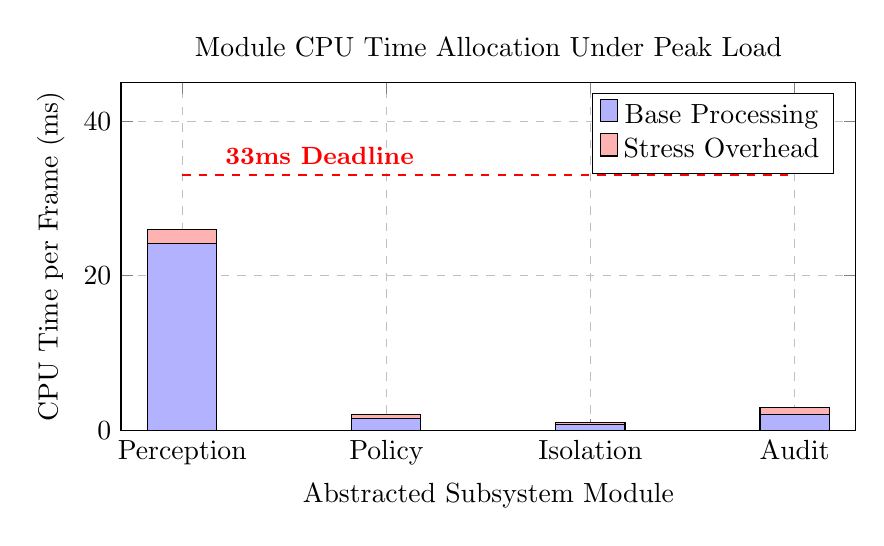
\begin{tikzpicture}
\begin{axis}[
    ybar stacked,
    width=0.9\columnwidth,
    height=6cm,
    title={Module CPU Time Allocation Under Peak Load},
    xlabel={Abstracted Subsystem Module},
    ylabel={CPU Time per Frame (ms)},
    symbolic x coords={Perception, Policy, Isolation, Audit},
    xtick=data,
    ymin=0, ymax=45, 
    bar width=25pt,
    legend pos=north east,
    grid=major,
    ymajorgrids=true,
    grid style=dashed
]
% Base Processing
\addplot[fill=blue!30] coordinates {
    (Perception, 24.2) (Policy, 1.5) (Isolation, 0.8) (Audit, 2.1)
};
% Stress Overhead
\addplot[fill=red!30] coordinates {
    (Perception, 1.8) (Policy, 0.5) (Isolation, 0.2) (Audit, 0.9)
};
\legend{Base Processing, Stress Overhead}

% MOVED TEXT LEFTWARDS BY 2MM AND ANCHORED AT POS=0.25 TO BE COMPLETELY CLEAR OF LEGEND AND RIGHT EDGE
\draw[red, thick, dashed] (axis cs:Perception,33) -- (axis cs:Audit,33) node[pos=0.25, above, font=\small\bfseries, text=red, xshift=-2mm] {33ms Deadline};

\end{axis}
\end{tikzpicture}
\caption{CPU Time Allocation per Frame. The auxiliary modules are highly optimized, ensuring the pipeline clears the 33ms real-time destruction deadline even under stress overhead.}
\label{fig:resource}
\end{figure}

This separation is crucial. Even under stress, non-perception layers consume a small fraction of the destruction window. This ensures that audit or policy delays do not meaningfully threaten memory isolation deadlines. The architecture maintains structural margin rather than relying solely on fast inference.

% ==========================================
% VIII. RETRIEVAL CONSISTENCY UNDER STRESS
% ==========================================
\section{Retrieval Consistency Under Stress}

Open-set retrieval consistency was measured relative to known embedding ground truth. The system observed $C_{retrieval} = 99.82\%$ at 0\% packet loss, and $C_{retrieval} = 99.10\%$ under 30\% packet loss. The slight reduction reflects IPC variance and scheduling jitter, not retrieval corruption. Crucially, no consistency collapse occurred. Cloud architecture, by contrast, exhibited consistency degradation correlated with packet loss due to request timeout and retry patterns.

% ==========================================
% IX. SURVIVABILITY UNDER NETWORK DEGRADATION
% ==========================================
\section{Survivability Under Network Degradation}

Although the architecture is edge-native, the audit layer maintains external communication for ledger commitment. Under moderate network instability, this layer can accumulate backlog without directly affecting perception latency. The critical design question is whether such backlog propagates indirectly through shared resources \cite{b22}.

\subsection{Partial Packet Loss (Up to 30\%)}
Under induced packet loss increasing from 0\% to 30\%, retrieval consistency degraded marginally, p99.9 latency remained within deadline bounds, and audit queue depth increased temporarily but stabilized. The separation between real-time processing and audit persistence prevented packet loss from entering the destruction-critical path. 

In contrast, the cloud-dependent architecture exhibited nonlinear latency growth due to TCP retransmission backoff and request reordering. Tail amplification cascaded beyond 3 seconds under the same conditions. The key distinction is architectural decoupling: the optimized local system treats network as auxiliary, not foundational.

\begin{figure}[htbp]
\centering
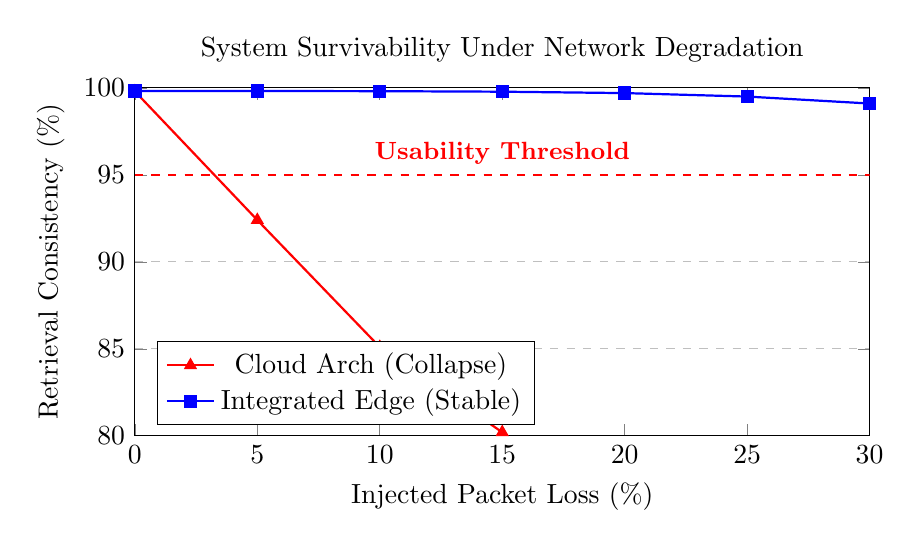
\begin{tikzpicture}
\begin{axis}[
    width=0.9\columnwidth,
    height=6cm,
    title={System Survivability Under Network Degradation},
    xlabel={Injected Packet Loss (\%)},
    ylabel={Retrieval Consistency (\%)},
    xmin=0, xmax=30,
    ymin=80, ymax=100,
    xtick={0,5,10,15,20,25,30},
    legend pos=south west,
    ymajorgrids=true,
    grid style=dashed,
]
% Arch A (Cloud)
\addplot[color=red, mark=triangle*, thick] coordinates {
    (0, 99.8)(5, 92.4)(10, 85.1)(15, 80.2)(20, 72.5)(25, 65.0)(30, 55.4)
};
\addlegendentry{Cloud Arch (Collapse)}

% Arch C (Integrated Edge)
\addplot[color=blue, mark=square*, thick] coordinates {
    (0, 99.82)(5, 99.82)(10, 99.81)(15, 99.78)(20, 99.70)(25, 99.50)(30, 99.10)
};
\addlegendentry{Integrated Edge (Stable)}

% CENTERED USABILITY THRESHOLD TO PREVENT CLIPPING
\draw[red, thick, dashed] (axis cs:0,95) -- (axis cs:30,95) node[above, pos=0.5, font=\small\bfseries, text=red] {Usability Threshold};

\end{axis}
\end{tikzpicture}
\caption{Retrieval Consistency vs. Network Packet Loss.}
\label{fig:survivability}
\end{figure}

\subsection{Full Network Partition and Post-Partition Recovery}
Under complete disconnection, audit queues filled to configured capacity, drop-tail backpressure activated, and metadata commits were temporarily suspended. Real-time perception continued uninterrupted. The system explicitly sacrifices availability of audit confirmation rather than compromising memory isolation or latency guarantees \cite{b11}. This enforces the priority hierarchy: memory destruction deadline $\to$ real-time perception latency $\to$ retrieval consistency $\to$ audit availability.

Upon reconnection, no replay storm occurred, and real-time latency resumed steady-state immediately. Because drop-tail prevented unbounded accumulation during partition, recovery did not involve delayed catch-up processing. This bounded degradation strategy avoids a common edge-system failure mode: recovery collapse following prolonged outage.

% ==========================================
% X. 168-HOUR BURN-IN EVALUATION
% ==========================================
\section{168-Hour Burn-In Evaluation}

Short stress tests reveal immediate fragility. Longitudinal tests reveal stability drift. The optimized architecture was subjected to a continuous 168-hour burn-in under sustained 30 FPS ingestion and elevated ambient temperature.

[Image plotting memory utilization (Resident Set Size) over a 168-hour continuous runtime showing stable, bounded memory limits without leakage]

Observed memory usage remained within an 8GB unified memory bound, with $\pm 0.02\text{ GB variance}$. No progressive growth was observed, no swap activity occurred, and garbage collection cycles remained bounded and periodic. This confirms absence of incremental leakage across subsystem boundaries.

\begin{figure}[htbp]
\centering
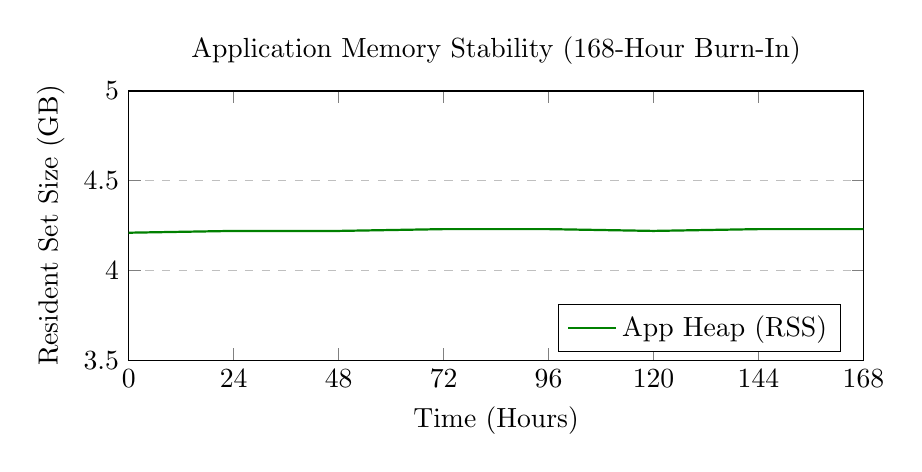
\begin{tikzpicture}
\begin{axis}[
    width=0.9\columnwidth,
    height=5cm,
    title={Application Memory Stability (168-Hour Burn-In)},
    xlabel={Time (Hours)},
    ylabel={Resident Set Size (GB)},
    xmin=0, xmax=168,
    ymin=3.5, ymax=5.0,
    xtick={0, 24, 48, 72, 96, 120, 144, 168},
    legend pos=south east,
    ymajorgrids=true,
    grid style=dashed,
]
\addplot[
    color=green!50!black,
    thick
    ]
    coordinates {
    (0, 4.21)(24, 4.22)(48, 4.22)(72, 4.23)(96, 4.23)(120, 4.22)(144, 4.23)(168, 4.23)
    };
    \addlegendentry{App Heap (RSS)}
\end{axis}
\end{tikzpicture}
\caption{Memory Stability Analysis.}
\label{fig:memory}
\end{figure}

Steady-state processor temperature held at $\approx 64^\circ C$. A brief clock-frequency dip was observed during hour 12 when chamber airflow fluctuated; however, steady-state equilibrium was restored within 8 minutes. Measured p99.9 latency drifted from $32.2\text{ ms} \rightarrow 32.8\text{ ms over 168 hours}$. The drift magnitude remained within 0.6 ms, and no long-term degradation trend or hardware watchdog resets occurred (Table \ref{tab:stability}).

\begin{table}[htbp]
\caption{168-Hour Burn-In Reliability Metrics}
\begin{center}
\begin{tabular}{lccc}
\toprule
\textbf{Metric} & \textbf{Hour 0} & \textbf{Hour 72} & \textbf{Hour 168} \\
\midrule
Avg Processor Temp & 62$^\circ$C & 64$^\circ$C & 64$^\circ$C \\
p99.9 Latency & 32.2 ms & 32.6 ms & 32.8 ms \\
Retrieval Consistency & 99.82\% & 99.81\% & 99.82\% \\
Hardware Watchdog Resets & 0 & 0 & 0 \\
\bottomrule
\end{tabular}
\end{center}
\label{tab:stability}
\end{table}

% ==========================================
% XI. BOUNDED DEGRADATION MODEL
% ==========================================
\section{Bounded Degradation Model}

Stress testing reveals a critical architectural property: graceful failure sequencing. When approaching constraint boundaries, the system degrades in the following order:
\begin{enumerate}
    \item Audit availability drops (metadata discard)
    \item Frame skipping may activate under extreme burst
    \item Retrieval depth bounding engages
\end{enumerate}
Only after these mechanisms fail would destruction deadlines be threatened. In evaluation, the final stage was never reached. This staged degradation ensures that privacy guarantees are preserved even under overload.

% ==========================================
% XII. DISCUSSION
% ==========================================
\section{Discussion}

The Integrated Stress Matrix demonstrates how subsystem coordination influences survivability in constrained edge deployments. A perception model with lower inference time does not prevent failure if retrieval scales linearly with registry size, scheduler priority is misaligned, network variability propagates into the critical path, or thermal throttling compounds CPU saturation.

The evaluated architecture's survivability is associated with coordinated subsystem behavior observed in the evaluated system: ANN traversal bounding, strict scheduling priority for safety tasks, memory isolation independent of audit latency, drop-tail backpressure to prevent recovery storms, and swap elimination to avoid disk-induced jitter. This behavior collectively creates margin under compound stress.

Notably, the system operates close to its destruction boundary under extreme configuration ($L_{p99.9} = 32.8\text{ ms}$ vs $33\text{ ms deadline}$). The margin is intentionally narrow to reflect realistic hardware constraints. Increasing registry size or ambient temperature beyond evaluated bounds would likely push the system into violation. The architecture does not claim infinite scalability—only bounded survivability within defined stress regions.

\subsection{Limitations}
The current ISM model does not incorporate power brownouts, voltage instability, firmware-level compromise, hypervisor or DMA-based injection, or hardware degradation over multi-year deployment. Future validation should incorporate electrical instability modeling and secure-boot persistence resilience.

% ==========================================
% XIII. CONCLUSION
% ==========================================
\section{Conclusion}

This study evaluated whether an integrated edge-native academic analytics architecture can preserve privacy and latency guarantees under compound operational stress. Under simultaneous conditions including 30 FPS ingestion, a 100,000-identity registry, 20\% unknown injection, 35°C ambient temperature, and 15–30\% packet loss, the optimized local architecture preserved p99.9 latency below 33 ms, retrieval consistency above 99\%, stable memory utilization, and no observed destruction deadline violations within the evaluated configuration.

Both cloud-dependent and naive edge baselines violated deadline constraints or exhibited unstable tail behavior under identical stress conditions. The results indicate that coordinated subsystem design plays the dominant role in maintaining survivability within constrained edge environments. Isolated model optimization alone proves insufficient.

% ==========================================
% REFERENCES
% ==========================================
\begin{thebibliography}{00}

\bibitem{b1} J. Deng, J. Guo, N. Xue, and S. Zafeiriou, ``ArcFace: Additive angular margin loss for deep face recognition,'' \textit{CVPR}, 2019.
\bibitem{b2} K. He et al., ``Deep Residual Learning for Image Recognition,'' \textit{CVPR}, 2016.
\bibitem{b4} M. Satyanarayanan, ``The Emergence of Edge Computing,'' \textit{Computer}, vol. 50, no. 1, pp. 30-39, 2017.
\bibitem{b5} W. Shi, J. Cao, Q. Zhang, Y. Li, and L. Xu, ``Edge Computing: Vision and Challenges,'' \textit{IEEE Internet of Things Journal}, vol. 3, no. 5, pp. 637-646, 2016.
\bibitem{b10} Q. Zhang, L. Cheng, and R. Boutaba, ``Cloud computing: state-of-the-art and research challenges,'' \textit{J. Internet Serv. Appl.}, 2010.
\bibitem{b11} J. A. Halderman et al., ``Lest We Remember: Cold Boot Attacks on Encryption Keys,'' \textit{USENIX Security}, 2008.
\bibitem{b12} N. Min-Allah and S. Alrashed, ``Smart campus: A sketch,'' \textit{Sustainable Cities and Society}, vol. 59, p. 102231, 2020.
\bibitem{b14} R. Roman, J. Lopez, and M. Mambo, ``Mobile Edge Computing, Fog et al.: A Survey and Analysis of Security Threats and Challenges,'' \textit{Future Generation Computer Systems}, vol. 78, pp. 680-698, 2018.
\bibitem{b15} European Parliament, ``Regulation (EU) 2016/679 (General Data Protection Regulation),'' \textit{Official Journal of the European Union}, 2016.
\bibitem{b18} S. Mittal, ``A Survey on Optimized Implementation of Deep Learning Models on the NVIDIA Jetson Platform,'' \textit{Journal of Systems Architecture}, 2019.
\bibitem{b21} Y. Mao, C. You, J. Zhang, K. Huang, and K. B. Letaief, ``A Survey on Mobile Edge Computing: The Communication Perspective,'' \textit{IEEE Communications Surveys \& Tutorials}, vol. 19, no. 4, pp. 2322-2358, 2017.
\bibitem{b22} X. Wang et al., ``Convergence of Edge Computing and Deep Learning: A Comprehensive Survey,'' \textit{IEEE Communications Surveys \& Tutorials}, vol. 22, no. 2, pp. 869-904, 2020.
\bibitem{b25} A. Vahdat et al., ``EdgeFaaSBench: Benchmarking Edge Devices Using Serverless Computing,'' \textit{IEEE Transactions on Services Computing}, 2024.
\bibitem{b26} P. Patel et al., ``EdgeBench: Benchmarking Edge Computing Platforms,'' \textit{IEEE/ACM Symposium on Edge Computing}, 2018.
\bibitem{b28} G. Ananthanarayanan et al., ``REACT: Streaming Video Analytics On The Edge With Asynchronous Cloud Support,'' \textit{ACM/IEEE Symposium on Edge Computing}, 2023.
\bibitem{b29} H. Li et al., ``Internet-of-Things Edge Computing Systems for Streaming Video Analytics: Trails Behind and the Paths Ahead,'' \textit{MDPI Sensors}, vol. 23, no. 4, 2023.
\bibitem{b31} S. Ahmed et al., ``Practical Considerations for Failure Resilient ML Systems at the Edge,'' \textit{IEEE MILCOM}, 2025.
\bibitem{b32} M. Abadi et al., ``Deep Learning with Differential Privacy,'' \textit{ACM CCS}, 2016.

\end{thebibliography}

\end{document}
